\documentclass[runningheads]{llncs}
\usepackage{graphicx}
\graphicspath{ {./images/} }
\begin{document}
\title{Raportul tehnic al proiectului 'My2FA'}
\author{Gavril Octavian (2A5)}
\authorrunning{Gavril Octavian 2A5}
\institute{Facultatea de Informatică, Universitatea “Alexandru Ioan Cuza”, Strada General Berthelot, nr. 16, Oras IAŞI, Cod Postal 700483, ROMANIA
\email{secretariat@info.uaic.ro}\\
\url{https://www.info.uaic.ro/}}

\maketitle              

\begin{abstract}
Acest raport a fost creat cu scopul de a prezenta cum functioneaza proiectul 'My2FA' si cum a fost acesta gandit. 

\keywords{C \and TCP/IP \and Socket}
\end{abstract}

\begin{figure}
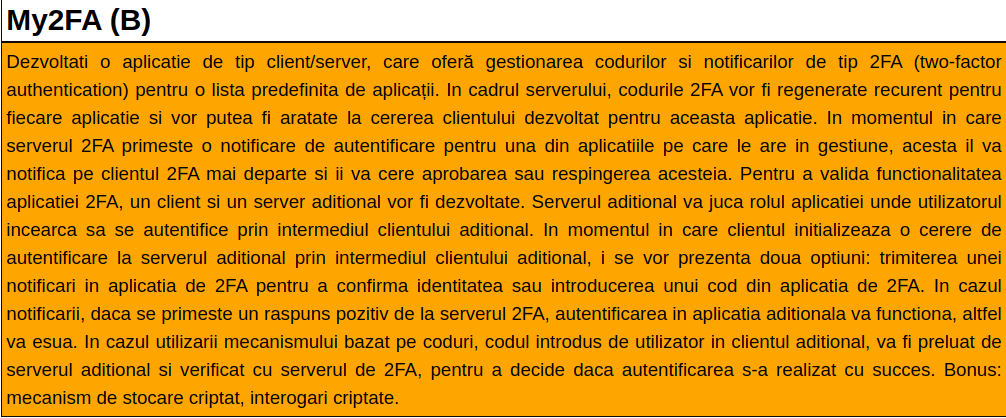
\includegraphics[width=\textwidth]{enunt}
\caption{Enuntul proiectului}
\end{figure}
\vspace{4cm}
\section{Introducere}

\hspace{10pt} Proiectul My2FA consta intr-o aplicatie de tipul client/server cu ajutorul careia clientul se poate autentifica in 2 pasi la orice alta aplicatie gestionata de sever-ul principal. Fiecare client va mentiona totodata si aplicatia la care doreste sa se autentifice iar dupa logarea cu username si parola acesta va putea alege, ca mecanism 2FA, intre a confirma identitatea sau a introduce codul 2FA generat pentru finalizarea actiunii de autentificare. Server-ul poate accepta oricati clienti dupa ce s-a realizat conexiunea cu aplicatiile din lista predefinita a acestuia.

\section{Tehnologii utilizate}
\subsection{Limbajul folosit}
\hspace{10pt} Aplicatia 'My2FA' a fost construita in limbajul de programare C.
\subsection{Modelul client/server}
\hspace{10pt} Ca model de interactiune intre client si server am ales sa-l folosesc pe cel orientat-conexiune, bazat pe TCP. Am abordat o implementare concurenta, server-ul putand procesa cererile mai multor clienti dar si cererile mai multor servere aditionale (in limita listei predefinite). Toate cele mentionate anterior au fost create cu ajutorul socket-urilor, intrucat ofera suport pentru diferite protocoale de comunicatie, inclusiv TCP. Mai mult, se obtine un suport pentru comunicatii orietate-conexiune si prin mesaje, ceea ce ofera garantia unei conexiuni sigure, necesara atat intre client si server, client si client aditional, client aditional si server aditional dar si intre server si server-ul aditional.
\subsection{Multitasking}
\hspace{10pt} Pentru implementarea server-ului per-client process am folosit thread-uri, astfel incat se creeaza cate un fir de executie pentru a servi unui anumit client cu un anumit server aditional iar numarul de clienti nu este limitat. Am ales sa folosesc thread-uri inloc de o abordare cu procese pentru a obtine costuri minime ale procesorului si un timp de executie mai mic. Un alt motiv pentru care am ales lucrul cu thread-uri este nevoia de lucru cu variabile globale, intrucat firele de executie impart aceeasi memorie.
\subsection{Stocarea datelor}
\hspace{10pt} Pentru stocarea numelor aplicatiilor gestionate de server cat si username-urile cu parolele aferente ce sunt inregistrate in server-ul aplicatiei aditionale am folosit fisiere de tip text (apps.txt si users.txt). De asemenea, pentru fiecare aplicatie am creat cate o structura globala ce contine datele specifice fiecarei aplicatii (numarul de clienti, vectorul de clienti, descriptorul de comunicare cu aplicatia, etc.).\\
\vspace{1cm}
	
	
\section{Arhitectura aplicatiei}
\subsection{Conceptele implicate}
\hspace{10pt} Structura aplicatiei 'My2FA' este reprezentata de conexiunea client-server la care se adauga si clientul aditional impreuna cu server-ul aditional ce joaca rol de aplicatie. In esenta, principalele actiuni dintre client si server constau in:
\begin{itemize}
	\item Instiintarea server-ului in legatura cu aplicatia in care doreste sa se autentifice clientul.
	\item Cererea clientului a unui cod 2FA generat de server pentru aplicatia respectiva, ce ulterior este introdus de catre utilizator in clientul aditional.
	\item Cererea server-ului pentru confirmarea identitatii clientului.
\end{itemize}
\hspace{10pt} Intregul procedeu este monotorizat de catre server-ul aditional ce asigura ca niciun pas al autentificarii sa nu fie omis. Astfel, interactiune clientului cu aplicatia este restrictionata, nefiind permisa orice comanda. Astfel, singura comanda recunoscuta in mod special este comanda '\textbf{Get code}' cu ajutorul careia clientul va obtine codul 2FA ce ii este destinat conectarii cu aplicatia aditionala.\\

Pe langa toate acestea, apar in structura aplicatiei si urmatoarele operatiuni:
\begin{itemize}
	\item Intreaga conexiune dintre client si server aditional se realizeaza prin clientul aditional.
	\item Server-ul aditional verifica, cu ajutorul server-ului 2FA, informatiile trimise de client (codul 2FA, confirmarea identitatii).
	\item Orice raspuns din partea server-ului aditional de tipul 'Login success!' sau 'Login failed!' va duce la terminarea programului client.
\end{itemize}

\vspace{2cm}
\subsection{Diagrama aplicatiei}
\hspace{10pt} Pentru o viziune mai clara a structurii aplicatiei 'My2FA' am pregatit urmatoarea diagrama:

\begin{figure}
\center 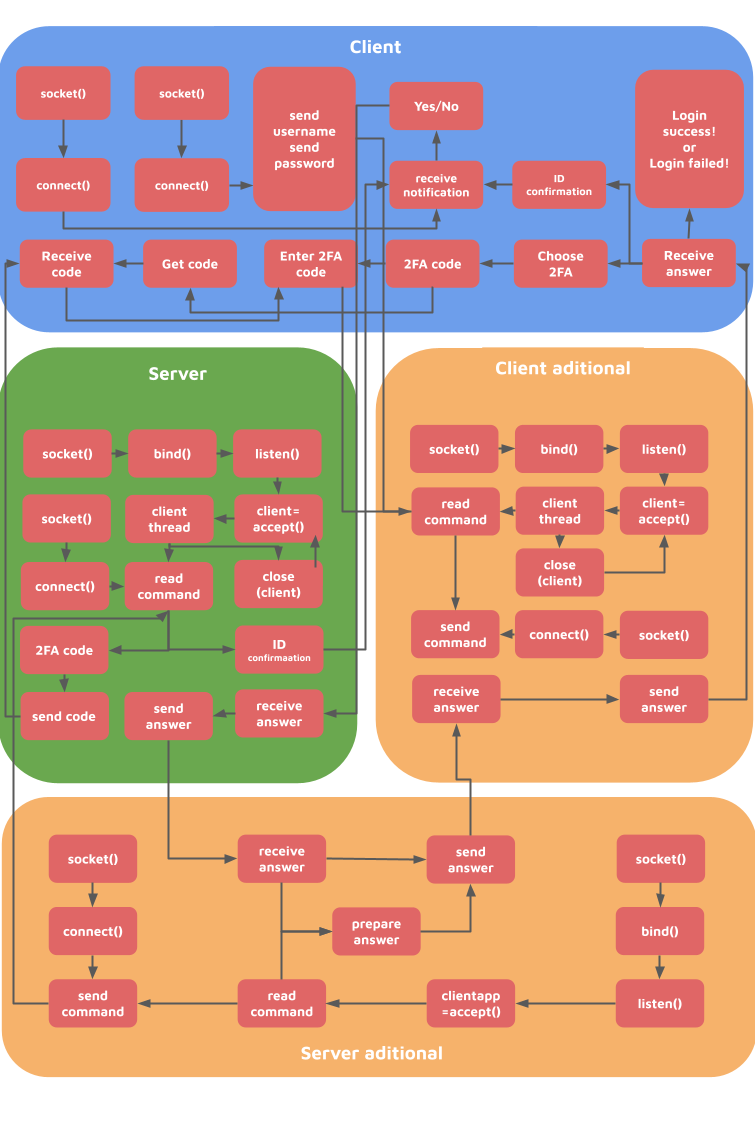
\includegraphics[width=315pt]{diagrama}
\caption{Diagrama aplicatiei}
\end{figure}

\section{Detalii de implementare}
\subsection{Evidenta necesitatii de comunicare cu server-ul a clientului pentru primirea notificarii cat si pentru obtinerea codului 2FA (client.c)}
	\begin{verbatim}
	...
   if (strcmp(msg, "For the 2nd FA, do you want to confirm your 
   ID or enter the 2FA code?") == 0 || strcmp(msg, "Invalid 
   command!\nFor the 2nd FA, do you want to confirm your ID or
   enter the 2FA code?") == 0) // evidenta necesitatii 
   conexiunii cu server-ul
      {
        serv_conn = 1;
        printf("%s\n", msg);
      }
      else if (strcmp(msg, "[If you don't know your 2FA code 
      type 'Get code']\nEnter 2FA code:") == 0 || strcmp(msg,
      "Invalid command\n[If you don't know your 2FA code 
      type 'Get code']\nEnter 2FA code:") == 0)
      {
        printf("%s\n", msg);
        need_code=1;
      }
      else if (strcmp(msg, "Login success!") == 0 || 
      strcmp(msg, "Login failed!") == 0)
      {
        printf("%s\n", msg);
        break;
      }
      else
        printf("%s", msg);
        ....
\end{verbatim}
\subsection{Functia de generare de coduri 2FA folosita de server (server.c)}
	\begin{verbatim}
	...
char *code_generator(char *code)
{
	srand(time(NULL));
	char alphabet[62] = {'a', 'b', 'c', 'd', 'e', 'f', 'g',
	'h', 'i', 'j', 'k', 'l', 'm', 'n','o', 'p', 'q', 'r',
	's', 't', 'u', 'v', 'w', 'x', 'y', 'z','A', 'B', 'C',
	'D', 'E', 'F', 'G', 'H', 'I', 'J', 'K', 'L', 'M', 'N',
	'O', 'P', 'Q', 'R', 'S', 'T', 'U', 'V', 'W', 'X', 'Y',
	'Z','0', '1', '2', '3', '4', '5', '6', '7', '8', '9'};
	for (int i = 0; i < 6; i++)
		code[i] = alphabet[rand() % 62];
	code[6] = '\0';
	return code;
}
    ...
\end{verbatim}
\subsection{Preluarea mesajelor server-ului aditional codificate asa incat se stie carui client trebuie trimis mesajul (clientapp.c)}
	\begin{verbatim}
	...
char msg[100] = "";
			bzero(msg, 100);
			if (read(tdL.app, msg, 100) == -1)
			{
				printf("eroare la primirea mesajului1!\n");
				return errno;
			}
			else
			{
				char id[10] = "";
				strcpy(id, extract_id(msg));
				strcpy(msg, extract_comanda(msg));
				printf("Am primit mesajul: '%s'\n", msg);
				if (write(clients[atoi(id)], msg, 100) < 0)
				{
					perror("[clientapp]Eroare la write() spre client.\n");
					return errno;
				}
				printf("Am scris catre id = %s din id = %d\n", id, tdL.idThread);
			}
	...
\end{verbatim}
\subsection{Monitorizarea tuturor pasilor de catre server-ul aditional pentru efectuarea in intregime a procesului de autentificare si prelucrarea datelor in mod corespunzator(serverapp.c)}
	\begin{verbatim}
	...
	else if (strcmp(tdL.s, "2FA code") == 0 && clients[atoi(id)].pas3
	 == 0 && clients[atoi(id)].pas2 == 1)
    {
        printf("cerem codul 2FA\n");
        bzero(msg, 100);
        clients[atoi(id)].pas3 = 1;
        strcpy(msg, "[If you don't know your 2FA code type 'Get code']
        \nEnter 2FA code:");
        strcpy(ultim_rasp, msg);
        strcat(msg, "/");
        strcat(msg, id);
        if (write(tdL.cl, msg, 100) < 0)
        {
            printf("eroare la scrierea mesajului eroare\n");
            exit(1);
        }
        printf("%s\n", msg);

        bzero(msg, 100);
        strcpy(msg, "2FA code/");
        strcat(msg, id);

        if (write(tdL.sv, msg, 100) < 0)
        {
            printf("eroare la scrierea mesajului eroare\n");
            exit(1);
        }

        bzero(msg, 100);
        if (read(tdL.sv, msg, 100) < 0)
        {
            perror("eroare la citire cod din server.\n");
            return errno;
        }
        strcpy(clients[atoi(id)].cod, msg);
        printf("Am primit codul din mesajul: %s\n", 
    }
    ...
\end{verbatim}
\subsection{Scenarii de utilizare}
\hspace{10pt} Un scenariu de utilizare poate fi folosirea aplicatie My2FA pentru conectarea pe aplicatii precum Facebook, Steam, Google, asa incat ar aduce o protectie in plus asupra contului unui client cat si asupra datelor acestuia.
\section{Concluzii}
\subsection{Remarci}
\hspace{10pt} Putem spune, fara indoiala, ca cel mai important aspect al acestei aplicatii este comunicarea dintre membrii acesteia. Functionalitatea aplicatiei depinde de sincronizarea dintre citirile si scrierile mesajelor dintre programe. 
\subsection{Posibile imbunatatiri}
\hspace{10pt} O imbunatatire ar putea fi posibilitatea de conectarea a oricator aplicatii la server. De asemenea, stocarea datelor clientilor cu privire la codul 2FA sau descriptorul de scriere ar fi mai sigura daca am folosi o baza de date care nu depinde de server.

\renewcommand\refname{Bibliografie}
\begin{thebibliography}{8}
\bibitem{ref_url1}https://profs.info.uaic.ro/~computernetworks/cursullaboratorul.php
\bibitem{ref_url2}https://profs.info.uaic.ro/~georgiana.calancea/laboratories.html 
\end{thebibliography}
\end{document}
